%
%===============>>  ГРУППА 6-1 МОДУЛЬ 7  <<=============
%
\setmodule{7}

%BEGIN_FOLD % ====>>_____ Занятие 1 _____<<====
\begin{class}[number=1]
	\begin{definit}
		Обе части уравнения можно умножить или разделить на одно и то же число, не равное нулю. Слагаемое можно перенести из одной части уравнения в другую, изменив его знак на противоположный.
	\end{definit}
	\begin{listofex}
		\item Решите уравнения: % 5.21(a-и) и 5.24 a в
		\begin{tasks}(2)
			\task \( x+0,9=1,5 \)
			\task \( 2-x=0,3 \)
			\task \( x-3,8=1,4 \)
			\task \( 0,8-x=1,3 \)
			\task \( 2-x=0,3 \)
			\task \( -0,5+x=3,4 \)
			\task \( x-3,6=-5 \)
			\task \( 9-7y=25-3y \)
			\task \( 4x=0 \)
			\task \( -2y=0 \)
			\task \( -40 \cdot (-7+5)=-1600 \)
			\task \( -2,1 \cdot (4-6y)=-42 \)
		\end{tasks}
		\item Решите уравнение, используя основное свойство пропорции:
		\begin{tasks}(2)
			\task \( \dfrac{-3}{9-4a} = \dfrac{40}{200} \)
			\task \( \dfrac{x-3}{6} = \dfrac{7}{3} \)
			\task \( \dfrac{1-2b}{4} = \dfrac{0,8}{0,5} \)
			\task \( \dfrac{5}{2x+3} = \dfrac{2,5}{4,5} \)
		\end{tasks}
		\item Решите уравнения: % 5,28(а-л) 
		\begin{tasks}(2)
			\task \( 11x=36-x \)
			\task \( 9x+4=48-2x \)
			\task \( 8-4x=2x-16 \)
			\task \( 0,4x+3,8=2,6-0,8x \)
			\task \( 6,8-1,3x=0,6x-2,7 \)
			\task \( \dfrac{4}{9}x+14=\dfrac{1}{6}x+9 \)
			\task \( 6x=28-x \)
			\task \( 9x-26=30-5x \)
			\task \( 7-3x=6x-56 \)
			\task \( 0,9x-7,4=-0,4x+4,3 \)
			\task \( 5,8-1,6x=0,3x-1,8 \)
			\task \( \dfrac{3}{8}x+19=\dfrac{7}{12}x+24 \)
		\end{tasks}
		\item Решите уравнение: % 5.30 ц
		\begin{tasks}
			\task \( \dfrac{1}{3} \left( \dfrac{1}{2}z+\mfrac{19}{1}{2} \right) = \left(  \mfrac{2}{7}{9}+\mfrac{3}{1}{3} \right) \cdot \dfrac{3}{5} \)
		\end{tasks}
	\end{listofex}
\end{class}
%END_FOLD

%%BEGIN_FOLD % ====>>_____ Занятие 2 _____<<====
%\begin{class}[number=2]
%	\title{Подготовка к проверочной}
%	\begin{listofex}
%		\item Найдите сумму чисел, противоположных данным:
%		\begin{tasks}(2)
%			\task \( -25 \) и  \( \dfrac{-8}{2} \)
%			\task \( |-5| \) и \( 6,15 \)
%			\task \( -(7-16,2) \) и \( -24,7 \)
%			\task \( |-11 \cdot 2| \) и \( 14:(-7) \)
%		\end{tasks}
%		\item Вычислите:
%		\begin{tasks}(3)
%			\task \( 15 - 97 \)
%			\task \( 14,6-23,5 \)
%			\task \( -78,15 + 16,22 \)
%			\task \( |-8,5| - |-15,16| \)
%			\task \( -\dfrac{15}{-4} + |4,34| \)
%			\task \( -8 \cdot (-0,25)\)
%			\task \( 6,36 \cdot \dfrac{-1}{6} \)
%			\task \( \dfrac{-5}{16} \cdot (-0,8) \)
%			\task \( -28 : (-7) \)
%			\task \( 46 : (-|23|) \)
%			\task \( \dfrac{|-4|}{-|2|} \cdot 0,25 \)
%			\task \( -(-12 + 4) \cdot |-5,5| \)
%		\end{tasks}
%		\item Решите уравнения:
%		\begin{tasks}(2)
%			\task \( 85-x=25 \)
%			\task \( 11,6-x=35,11 \)
%			\task \( -\dfrac{4}{10}+x=-0,27 \)
%			\task \( -\left( -\dfrac{8}{15} + x \right) = -4 \)
%			
%			\task \( |-15|:(-3)=x+2 \)
%			\task \( |-9 + 14,76| = -x+28 \)
%			\task \( 0,5 \cdot x-16,3=- |-11-2| \)
%			\task \( \dfrac{1}{x} = -|6-25,3| \)
%			
%			\task \( \dfrac{18}{x} = \dfrac{3}{9} \)
%			\task \( \dfrac{x}{4} = -\dfrac{24}{11} \)
%			\task \( \dfrac{17}{x} = \dfrac{34}{-28} \)
%			\task \( \dfrac{-x}{15} = \left| -\dfrac{5}{6} \right| \)
%		\end{tasks}
%		\item Вычислите: %4.33 а ф м ы
%			%\task \( -(2,4+3,5)-(4,2+0,6-3,5)+2,4 \)
%			%\task \( -4 \cdot (-5)-(-30):6  \)
%			%\task \( -4,9:(-0,2 \cdot 0,3 - 0,1 ) \)
%			%\task \( 2,07 : (-2,3) - 13,13:(-1,3) \)
%			\[ \left( \mfrac{6}{8}{25}:(-1)-(-0,8)\cdot(-0,1)\right) : \left( -0,25:1,25 - \mfrac{1}{3}{5} : \left( -\mfrac{5}{1}{3} \right) \right) \]
%	\end{listofex}
%\end{class}
%%END_FOLD
%
%BEGIN_FOLD % ====>>_ Домашняя работа 1 _<<====
%\begin{homework}[number=1]
%	\begin{listofex}
%		\item Разделите число:
%		\begin{tasks}(2)
%			\task \( 156 \) в отношении \( 2:1 \)
%			\task \( 270 \) в отношении \( 5:3:2 \)
%			\task \( 2160 \) в отношении \( 4:5:6 \)
%			\task \( 1210 \) в отношении \( 2,5:4:5,5 \)
%		\end{tasks}
%		\item Вычислите:
%		\begin{tasks}(3)
%			\task \( -17 + 21 \)
%			\task \( -8,5 - 0,6 \)
%			\task \( \dfrac{1}{6} - 13,5 \)
%			\task \( -4 + \mfrac{7}{4}{5} \)
%			\task \( -17 + \dfrac{5}{-3} \)
%			\task \( -10,33 - (-11,72) \)
%			\task \( 15 \cdot (-4) \)
%			%\task \( -5 \cdot \dfrac{4}{-5} \)
%			%\task \( -11 \cdot (-0,5) \)
%			\task \( -\dfrac{1}{3} \cdot \mfrac{1}{1}{2} \)
%			\task \( -\dfrac{5}{3}\cdot \dfrac{-1}{-18} \)
%			
%			\task \( 14 : (-0,7) \)
%			\task \( 0,16 : (-0,4) \)
%			%\task \( 42 : (-3,5) \)
%			%\task \( -\dfrac{8}{25} : (-0,125) \)
%			\task \( 7,11 : (-711) \)
%		\end{tasks}
%		\item Решите уравнения:
%		\begin{tasks}(2)
%			\task \( \dfrac{-4}{x}=116 \)
%			\task \( -\dfrac{-y}{-18}=\dfrac{1}{3} \)
%			\task \( -15,6:y=\dfrac{3}{-11} \)
%			\task \( \dfrac{x}{-0,72}=1,2 \cdot 0,4 \)
%		\end{tasks}
%	\end{listofex}
%\end{homework}
%%END_FOLD
%
%%BEGIN_FOLD % ====>>_____ Занятие 3 _____<<====
%\begin{exam}
%	\begin{listofex}
%		\item Вычислите:
%		\begin{tasks}(2)
%			\task \( 0,7 \cdot (-22) \)
%			\task \( 0,25 - 16 \cdot 0,2 \)
%			\task \( |-0,4| - (-0,57) \)
%			\task \( -25,11 + 53,75 \)
%			\task \( \left| \mfrac{2}{4}{5} - 5 \right| \cdot (-2) \)
%			\task \( 14,4 : (-0,3) \)
%			\task \( 15,3 \cdot (-|-2|) - (-30) \)
%			\task \( \dfrac{18}{4} + 6 \cdot (-3,5) \)
%			\task \( |-16| : 4 + (-8) \)
%			\task \( -\dfrac{-|-15,5|}{5} - |-0,14+16,2| \)
%		\end{tasks}
%		\item Решите уравнения:
%		\begin{tasks}(2)
%			\task \( 15x=x-28 \)
%			\task \( 3x+5=-14-5x \)
%			\task \( 7-\dfrac{3}{5}x=|-18,5|-6x \)
%			%\task \( 0,25x-|-3,8| \cdot 2 = 2,6 - 0,8x \)
%			%\task \( 11,2-\dfrac{x}{25}=-0,6x+2,3 \)
%			\task \( \dfrac{4}{9}x-15=\dfrac{1}{-6}x-|12 \cdot (-0,5)| \)
%			%\task \( \dfrac{-7}{x} = \dfrac{-14}{-28} \)
%			\task \( \dfrac{x}{4} = \dfrac{3}{|-6|} \)
%			\task \( \dfrac{x-5}{-|5|} = \dfrac{10}{-0,5} \)
%			
%			\task \( \dfrac{-5x}{6} = \dfrac{15}{-0,12} \)
%			\task \( \dfrac{x-2}{14} = -\left( -\mfrac{1}{5}{8} \right) \)
%			\task \( \dfrac{-3}{9-4x} = \left| -\dfrac{40 \cdot (-1)}{-200} \right| \)
%		\end{tasks}
%		\item Вычислите: %4.33 ъ
%		\[ -\mfrac{3}{7}{20} + \left( -0,25 : (-0,25) - 1,5 : \left( -\dfrac{3}{16} \right) \right) : \left( -\mfrac{4}{1}{11} \right)  \]
%	\end{listofex}
%\end{exam}
%END_FOLD

%BEGIN_FOLD % ====>>_____ Занятие 2 _____<<====
\begin{class}[number=2]
	\begin{listofex}
		\item Вычислите:
		\begin{tasks}(2)
			\task \( 0,7 \cdot (-22) \)
			\task \( 0,25 - 16 \cdot 0,2 \)
			\task \( |-0,4| - (-0,57) \)
			\task \( -25,11 + 53,75 \)
			\task \( \left| \mfrac{2}{4}{5} - 5 \right| \cdot (-2) \)
			\task \( 14,4 : (-0,3) \)
			\task \( 15,3 \cdot (-|-2|) - (-30) \)
			\task \( \dfrac{18}{4} + 6 \cdot (-3,5) \)
			\task \( |-16| : 4 + (-8) \)
			\task \( -\dfrac{-|-15,5|}{5} - |-0,14+16,2| \)
		\end{tasks}
		\item Решите уравнения:
		\begin{tasks}(2)
			\task \( |x|=5 \)
			\task \( |x|=0 \)
			\task \( |x|=-2 \)
			\task \( |x+57|=13 \)
			\task \( |2x-13|=3 \)
			\task \( |4x-5|=9 \)
			\task \( \left| \dfrac{1}{3}x=5 \right|=6 \)
			\task \( \left| \dfrac{2x}{3}-9 \right|=9 \)
			\task \( \left| \dfrac{3}{4}x-\mfrac{1}{3}{7} \right|=\mfrac{2}{4}{9} \)
			\task \( ||x-1|-2|=3 \)
			\task \( 3|x|-8=9-4|x| \)
			\task \( 1-|23x-25|=7 \)
		\end{tasks}
	\end{listofex}
\end{class}
%END_FOLD

%BEGIN_FOLD % ====>>_ Домашняя работа 1 _<<====
\begin{homework}[number=1]
	\begin{listofex}
		\item Решите уравнения: % 5.21 й-р и 5.24 б г
		\begin{tasks}(2)
			\task \( 5x=3x \)
			\task \( -2n=5,7n \)
			\task \( 49x=50 \)
			\task \( x-156=16 \)
			\task \( -(11+x)=2,25 \)
			\task \( (-20x-50)\cdot 2 = 100 \)
			\task \( -3 \cdot (2-15x) = -6 \)
			\task \( -6x+2(5-3x)=8 \)
			\task \( |4-|x-5||-1=3 \)
			\task \( |5-|x+6||+1=6 \)
			\task \( 3|x|-5=10 \)
			\task \( |8-9x|=12 \)
		\end{tasks}
		\item Решите уравнение, используя основное свойство пропорции:
		\begin{tasks}(2)
			\task \( \dfrac{5+3x}{12} = \dfrac{4x-3}{18} \)
			\task \( \dfrac{0,9}{7+5y} = \dfrac{0,2}{y-4} \)
			\task \( \dfrac{x+7}{3} = \dfrac{2x-3}{5} \)
			\task \( \dfrac{0,2}{x+3} = \dfrac{0,7}{x-2} \)
		\end{tasks}
		\item Решите уравнение: % 5.30 щ ш
		\begin{tasks}
			\task \( \dfrac{1}{3} \left( \dfrac{5}{12}-4m \right) =\dfrac{4}{9} \left(  \mfrac{1}{1}{1} m-\dfrac{3}{8} \right) \)
			\task \( 0,3(5x-7)=3(0,2x+3,2) \)
		\end{tasks}
	\end{listofex}
\end{homework}
%END_FOLD

%BEGIN_FOLD % ====>>_____ Занятие 5 _____<<====
\begin{class}[number=5]
	\begin{listofex}
		\item Решите уравнения: %5.30 5.32(о ф ь)
		\begin{tasks}(2)
			\task \( 4x-x=24 \)
			\task \( 8x-8=20-6x \)
			\task \( 9-4x=3x-40 \)
			\task \( 0,6x-5,4=-0,8+5,8 \)
			\task \( 4,7-1,1x=0,5x-3,3 \)
			\task \( \dfrac{5x}{6}+16=\dfrac{4}{9}x+9 \)
			\task \( \dfrac{x}{2}+\dfrac{x}{3}+\mfrac{1}{5}{6}x=2 \)
			\task \( \dfrac{5x}{7}+\dfrac{x}{35}+x=-1 \)
			\task \( \dfrac{x}{2}+\dfrac{x}{3}+\dfrac{x}{4}=12 \)
			\task \( 0,18x-3,54=0,19x-2,89 \)
			\task \( \mfrac{2}{2}{5}x+ \mfrac{3}{2}{15}=\mfrac{3}{1}{5}x + \mfrac{2}{1}{3} \)
			\task \( \dfrac{1}{4} - \dfrac{1}{3}m=\mfrac{4}{1}{4}-3m \)
			\task \( \dfrac{-0,2(6x+1)}{3,6}=\dfrac{0,5x}{-9} \)
			\task \( \dfrac{3x-2,4}{0,02}=\dfrac{8-x}{0,1} \)
			\task \( \dfrac{3,6}{0,2(6y+1)}=\dfrac{9}{0,5y} \)
			\task \( \dfrac{1,4x-3,5}{0,25}=\dfrac{4,6x-18}{-1,5} \)
			\task \( 4(1,2x+3,7)=0,2(2,6x-14) \)
			\task \( 0,3(5x-7)=3(0,2x+3,2) \)
			\task \( \dfrac{x}{5}-4=-0,1x+2 \)
			\task \( 4,37+6,7x=7,75+9,3x \)
		\end{tasks}
		\item Решите уравнения: %5.36
		\begin{tasks}(2)
			\task \( |x|=5 \)
			\task \( |x|=0 \)
			\task \( |x|=-2 \)
			\task \( |x+57|=13 \)
			\task \( |2x-13|=3 \)
			\task \( |4x-5|=9 \)
			\task \( \left| \dfrac{1}{3}x=5 \right|=6 \)
			\task \( \left| \dfrac{2x}{3}-9 \right|=9 \)
			\task \( \left| \dfrac{3}{4}x-\mfrac{1}{3}{7} \right|=\mfrac{2}{4}{9} \)
			\task \( ||x-1|-2|=3 \)
			\task \( 3|x|-8=9-4|x| \)
			\task \( 1-|23x-25|=7 \)
		\end{tasks}
		
	\end{listofex}
\end{class}
%END_FOLD

%BEGIN_FOLD % ====>>_ Домашняя работа 1 _<<====
\begin{homework}[number=1]
	\begin{listofex}
		\item Решите уравнения: % 5.21 й-р и 5.24 б г
		\begin{tasks}(2)
			\task \( -2n=5,7n \)
			\task \( x-156=16 \)
			\task \( -(11+x)=2,25 \)
			\task \( (-20x-50)\cdot 2 = 100 \)
			\task \( -3 \cdot (2-15x) = -6 \)
			\task \( -6x+2(5-3x)=8 \)
			\task \( 3|x|-5=10 \)
			\task \( |8-9x|=12 \)
		\end{tasks}
		\item Решите уравнение, используя основное свойство пропорции:
		\begin{tasks}(2)
			\task \( \dfrac{5+3x}{12} = \dfrac{4x-3}{18} \)
			\task \( \dfrac{0,9}{7+5y} = \dfrac{0,2}{y-4} \)
			\task \( \dfrac{x+7}{3} = \dfrac{2x-3}{5} \)
			\task \( \dfrac{0,2}{x+3} = \dfrac{0,7}{x-2} \)
		\end{tasks}
		
	\end{listofex}
\end{homework}
%END_FOLD


%BEGIN_FOLD % ====>>_____ Занятие 6 _____<<====
\begin{class}[number=6]
	\begin{listofex}
		\item Занятие 6
	\end{listofex}
\end{class}
%END_FOLD

%BEGIN_FOLD % ====>>_ Домашняя работа 3 _<<====
\begin{homework}[number=3]
	\begin{listofex}
		\item Домашняя работа 3
	\end{listofex}
\end{homework}
%END_FOLD

%BEGIN_FOLD % ====>>_____ Занятие 7 _____<<====
\begin{class}[number=7]
	\title{Подготовка к проверочной}
	\begin{listofex}
		\item Занятие 7
	\end{listofex}
\end{class}
%END_FOLD

=%BEGIN_FOLD % ====>>_ Проверочная работа _<<====
\begin{exam}
	\begin{listofex}
		\item Проверочная
	\end{listofex}
\end{exam}
%END_FOLD

%BEGIN_FOLD% ====>>_ Консультация _<<====
\begin{consultation}
	\begin{listofex}
		\item Найдите значение выражения: \[ \dfrac{17}{20} - \dfrac{18}{25} \cdot \dfrac{5}{6} \]
		\item
		\begin{minipage}[t]{180pt}
			Найдите площадь трапеции \( ABCD \).
		\end{minipage}
		\hspace{0.01\linewidth}
		\begin{minipage}[t]{100pt}
			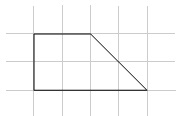
\includegraphics[align=t, width=\linewidth]{\picpath/61CONS-3}
		\end{minipage}
		
		%\item  с основаниями \(BC, AD\), если \(\angle ABC = \angle BAD = 90 \degree \) и \( AD=2AB=2BC=4 \).
		\item Килограмм кураги и чернослива стоят соответственно \(330\) рублей и \(410\) рублей. Покупатель взял полкилограмма кураги и полкилограмма чернослива и дал продавцу \(500\) рублей. Сколько рублей сдачи он должен получить.
		\item Коля летит рейсом из Якутска в Москву. В момент, когда пилот сообщил, что до посадки осталось \(2\) часа, Колины часы показывали \(19:50\) по Якутскому времени. Во сколько времени по местному времени сядет самолет? Часовой пояс Якутска --- МСК\(+6\).
		\item
		\begin{minipage}[t]{160pt}
		Пятеро друзей решили устроить вечер настольных игр. Каждый принёс свою игру, и все начали обсуждать, в какую игру они будут играть. Аня сказала, что не хочет играть в игру «Гонки на капибарах», которую принёс Боря, потому что Гена всегда в ней побеждает, а Гене не нравится игра «Всё о поездах», из-за которой в прошлый раз все поссорились. Вере очень нравится игра «Занятные мышата», но она не против поиграть и в другую игру, а Данила сказал, что ему без разницы и что он будет играть в любую игру, которую выберет большинство. Во что могут сыграть друзья этим вечером, чтобы все остались довольны? В таблице представлены ограничения по использованию для каждой из игр, которые есть у друзей.
		\end{minipage}
		\hspace{0.01\linewidth}
		\begin{minipage}[t]{140pt}
			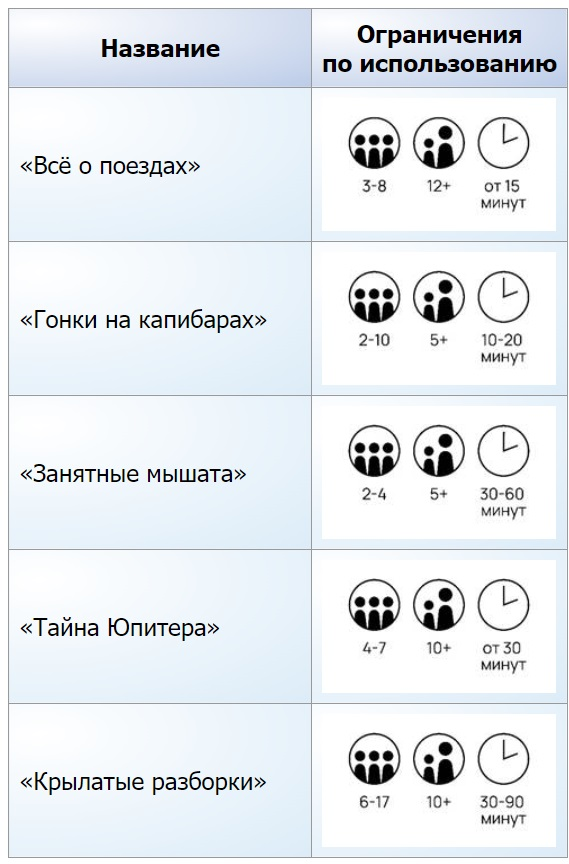
\includegraphics[align=t, width=\linewidth]{\picpath/61CONS}
		\end{minipage}
		
		%\begin{minipage}[t]{\bodywidth}
			\item Фанерозойский эон --- это временной промежуток «явной» жизни, который продолжается и сейчас. Некоторые учёные полагают, что он начался сразу после распада суперконтинета в конце глобального ледникового периода. На круговой диаграмме представлено разбиение фанерозойского эона на геологические периоды. Фанерозой длится уже около \(542\) млн лет и включает в себя эпоху динозавров. Динозавры жили на Земле в течение всей мезозойской эры (периоды триас, юра и мел). Теплый климат способствовал тому, чтобы рептилии господствовали и на суше, и в воде, и в воздухе. В конце мезозойской эры произошло массовое вымирание, в результате которого динозавры исчезли, а сохранились только их потомки --- птицы. Пользуясь диаграммой, определите, какую примерную долю рассмотренного времени на Земле жили динозавры. Выберите правильный вариант ответа.
		%\end{minipage}
		
		\hspace{0.1\linewidth}
		\begin{minipage}[c]{250pt}
			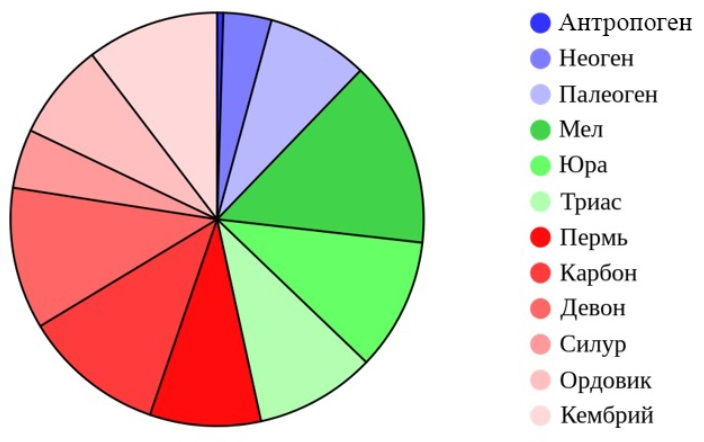
\includegraphics[align=t, width=\linewidth]{\picpath/61CONS-1}
		\end{minipage}
		\begin{tasks}(3)
			\task \( \dfrac{1}{2} \)
			\task \( \dfrac{1}{3} \)
			\task \( \dfrac{2}{3} \)
		\end{tasks}
		\item Во всех подъездах дома одинаковое число этажей, а на всех этажах одинаковое число квартир. При этом число этажей в доме больше числа квартир на этаже, число квартир на этаже больше числа подъездов, а число подъездов больше двух. Всего в доме \(84\) квартиры. В каком подъезде и на каком этаже находится квартира \(38\)?
		\item 
		\begin{minipage}[t]{200pt}
		Перед Вами карта Москвы. Москва подразделяется на 12 административных округов. При этом 8 из них названы по географическому признаку. Например, Южный административный округ (ЮАО) граничит с Юго-Западным (ЮЗАО) и Юго-Восточным (ЮВАО), а Юго-Восточный – с Южным и Восточным (ВАО) и т. д. Есть особый округ – Центральный, он граничит со всеми округами с географическими названиями, в нём находится большое количество достопримечательностей, исторический центр города, точка отсчёта расстояний (нулевой километр), Кремль. Зеленоградский административный округ не граничит ни с одним из округов. Не так давно к Москве присоединили ещё два округа: Новомосковский на юго-западе столицы (он граничит с ЮЗАО и ЗАО) и Троицкий (он граничит только с Новомосковским АО и является самым большим по площади из всех округов Москвы). Сколько округов Москвы граничит с Новомосковским административным округом?
		\end{minipage}
	\hspace{0.01\linewidth}
		\begin{minipage}[t]{110pt}
		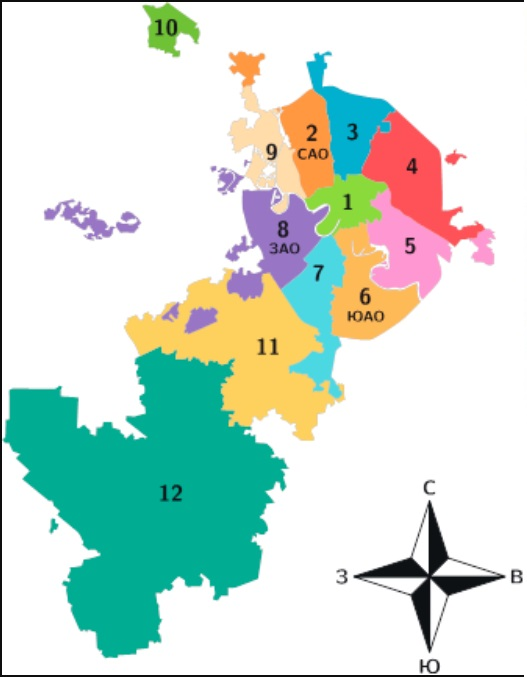
\includegraphics[align=t, width=\linewidth]{\picpath/61CONS-2}
		\end{minipage}
	\end{listofex}
\end{consultation}
%END_FOLD